\documentclass[10pt,a4paper,twocolumn]{article}

\usepackage[T1]{fontenc}
\usepackage{lmodern}
\usepackage[a4paper,top=2.2cm,bottom=2.2cm,left=2cm,right=2cm]{geometry}
\usepackage{amsmath}
\usepackage{graphicx}
\usepackage{float}
\usepackage{booktabs}
\usepackage{tabularx}
\usepackage{algorithm}
\usepackage{algpseudocode}
\usepackage{url}
\usepackage{microtype}
\usepackage{caption}
\usepackage{xcolor}
\usepackage{hyperref} % load last

% Figures: the generated PDFs, plus a folder for the board photo
\graphicspath{{../figures/generated/}{figures/}}

% Placeholder for numbers that come from the on-device held-out run (Part 4).
% Search for \TODO before submitting; none should remain.
\newcommand{\TODO}[1]{\textcolor{red}{\textbf{[#1]}}}
% Link to the demo video in the repository.
\newcommand{\VIDEOURL}{https://github.com/KD-CET/classification-pipeline/blob/main/media/demo_video.mov}

% ---------- spacing ----------
\setlength{\columnsep}{18pt}
\captionsetup{font=small,labelfont=bf,skip=6pt}
\captionsetup[table]{position=above,skip=6pt}
\setlength{\textfloatsep}{10pt plus 2pt minus 2pt}
\setlength{\dbltextfloatsep}{12pt plus 2pt minus 2pt}
\setlength{\floatsep}{8pt plus 2pt minus 2pt}
\setlength{\intextsep}{8pt plus 2pt minus 2pt}
\renewcommand{\topfraction}{0.9}
\renewcommand{\bottomfraction}{0.8}
\renewcommand{\textfraction}{0.1}
\renewcommand{\floatpagefraction}{0.8}
\renewcommand{\dbltopfraction}{0.9}
\renewcommand{\dblfloatpagefraction}{0.8}
\AtBeginDocument{%
  \setlength{\abovedisplayskip}{6pt plus 2pt minus 2pt}%
  \setlength{\belowdisplayskip}{6pt plus 2pt minus 2pt}%
  \setlength{\abovedisplayshortskip}{2pt plus 1pt}%
  \setlength{\belowdisplayshortskip}{4pt plus 1pt minus 1pt}%
}

\title{On-Device Lighting Classification with a Compact Table-Lookup Pipeline: A Proof of Concept on the ESP32}

\author{Kenneth Dialogo \\ Department of Computer Engineering Technology \\ Vanier College}

\date{October 17, 2026}

\begin{document}

\maketitle

\begin{abstract}
The previous lab proposed a table-lookup classifier, built offline with DBSCAN and per-class Gaussian kernel density estimation (KDE) and stored as one $16\times16$ byte table per class, and supported it with synthetic data only. This report tests the same pipeline on real measurements and on real hardware. An ESP32 reads a UV sensor (GUVA-S12SD) and the infrared channel of a TSL2591 light sensor, smooths both with an exponential moving average (EMA), and classifies the lighting as sun, shade, LED, or fluorescent, or answers UNKNOWN. Because the IR readings span more than two orders of magnitude, IR is log-transformed before scaling. On 2300 labelled readings, DBSCAN rediscovered the four lighting conditions without seeing the labels, with 100\% cluster purity. The shipped model occupies $K G^2 = 4\cdot16^2 = 1024$ bytes plus 16 bytes of scaling bounds, and the stored tables agreed with the continuous KDE on all 460 test points. On the ESP32, the device's decisions agreed with the desktop lookup on all 60 logged held-out readings, and the device classified LED, fluorescent, and dark-indoor readings as LED, fluorescent, and shade once the sensor was held still; while the sensor was still being positioned, agreement with the recorded label was much lower (35--48\%). Including the model added 2376 bytes of flash and 20 bytes of SRAM, and one lookup took 3.26~\textmu s, about 0.003\% of the 122~ms needed to take a sample. The main limitation is that the three indoor classes are separated by IR brightness alone, so the result depends on keeping the sensor geometry fixed.
\end{abstract}

% =====================================================================
\section{Proposed Pipeline}

The system separates model construction from inference. The offline stage runs once, on a workstation: feature transformation and scaling, DBSCAN clustering, KDE fitting, peak normalisation, and conversion of the maps into byte tables. A script then writes those tables, the training scaling bounds, the class names, and the reject threshold into a C header, \texttt{model.h}, which is compiled into the firmware. The device never sees the training data or repeats any offline step.

On the device, each sample first passes through the same filter used during data collection, an exponential moving average with $\alpha = 0.2$:
\begin{equation}
s_n = \alpha\, r_n + (1-\alpha)\, s_{n-1},
\label{eq:ema}
\end{equation}
where $r_n$ is the raw reading and $s_n$ the filtered one. The filtered readings are turned into the two features
\begin{equation}
x = s^{\mathrm{UV}}, \qquad y = \log_{10}\!\left(1 + s^{\mathrm{IR}}\right).
\label{eq:features}
\end{equation}
The logarithm is the one change to the feature space relative to the previous lab; Section~\ref{sec:method} explains why it is needed. The features are then scaled with the bounds computed from the training set,
\begin{equation}
\tilde{x} = \frac{x-x_{\min}}{x_{\max}-x_{\min}},
\qquad
\tilde{y} = \frac{y-y_{\min}}{y_{\max}-y_{\min}},
\label{eq:scale}
\end{equation}
and mapped to a grid cell,
\begin{equation}
\mathrm{col} = \left\lfloor \tilde{x}G \right\rfloor,
\qquad
\mathrm{row} = \left\lfloor \tilde{y}G \right\rfloor,
\label{eq:index}
\end{equation}
with both indices clipped to $[0,G-1]$. For each class $c$ the stored byte is read back as
\begin{equation}
\tilde{g}_c = \frac{Q_c[\mathrm{row},\mathrm{col}]}{255}.
\label{eq:dequant}
\end{equation}
The winning class is the one with the largest value; if that value is below $\tau=0.12$ the device reports UNKNOWN. Algorithm~\ref{alg:lookup} gives the complete loop as implemented. It reads $K$ bytes and performs $K$ comparisons per sample, so its cost does not depend on how much data trained the tables.

\begin{algorithm}[!bt]
\caption{On-device inference loop (ESP32).}
\label{alg:lookup}
\begin{algorithmic}[1]
\Require byte tables $Q_c$ in flash; training bounds $(x_{\min},x_{\max})$, $(y_{\min},y_{\max})$; grid size $G$; threshold $\tau$; filter constant $\alpha$
\Ensure a class name or \textsc{unknown}, at 5--10~Hz
\Loop
  \State read raw UV $r^{\mathrm{UV}}$ (ADC) and raw IR $r^{\mathrm{IR}}$ (TSL2591)
  \State $s \gets \alpha r + (1-\alpha) s$ for both signals \Comment{same filter as collection}
  \State $x \gets s^{\mathrm{UV}}$;\; $y \gets \log_{10}(1+s^{\mathrm{IR}})$
  \State $\tilde{x}\gets(x-x_{\min})/(x_{\max}-x_{\min})$;\; $\tilde{y}\gets(y-y_{\min})/(y_{\max}-y_{\min})$
  \State $\mathrm{col}\gets\lfloor\tilde{x}G\rfloor$, $\mathrm{row}\gets\lfloor\tilde{y}G\rfloor$, both clipped to $[0,G-1]$
  \For{each class $c$}
    \State $v_c\gets \texttt{pgm\_read\_byte}(Q_c[\mathrm{row},\mathrm{col}])/255$
  \EndFor
  \State $\hat{c}\gets\arg\max_c v_c$
  \If{$v_{\hat{c}}<\tau$}
    \State report \textsc{unknown}
  \Else
    \State report class name $\hat{c}$
  \EndIf
\EndLoop
\end{algorithmic}
\end{algorithm}

The filter and the logarithm are part of the model, not preprocessing details: the tables were built from filtered, log-transformed readings, so a device that skips either step would index the wrong cells. The firmware therefore uses the same $\alpha$, sensor gain, and integration time as the collection firmware.

% =====================================================================
\section{Application}

The target application is a lighting-condition node for daylight-harvesting control: a small sensor on a desk or window ledge that reports whether a space is lit by direct sun, outdoor shade, LED, or fluorescent light, so that blinds and artificial lighting can be adjusted without a person in the loop. The node sends a single class label (or UNKNOWN) rather than streaming raw readings.

Three properties of this application match the pipeline. First, unlabelled readings are easy to collect continuously, while labelled ones require someone to note the conditions, which is why the classes are discovered by clustering and only checked against labels afterwards. Second, the light sources differ in spectrum: only sunlight contains significant UV, and the sources differ in how much infrared they emit, so UV and IR together carry the information needed. Third, the decision must run continuously on a low-cost microcontroller.

The prototype runs on an ESP32-WROOM module, which has 4~MB of flash, so the 1040-byte model is not memory-critical here; it is about 0.025\% of flash. The point of the measurement is that the cost is known exactly before deployment and stays fixed, so the same model would also fit a much smaller part.

% =====================================================================
\section{Materials and Method}
\label{sec:method}

\paragraph{Hardware.} An ESP32 development board read a GUVA-S12SD UV module on GPIO34 (an ADC1 pin, 12-bit, 0--4095) and a TSL2591 light sensor over I\textsuperscript{2}C (SDA 21, SCL 22), both powered at 3.3~V. The assignment specified an IR photodiode in a voltage divider; that photodiode was non-functional, and per the instructor's direction the TSL2591 was used instead, reading its IR-only channel (16-bit) as the second sensor. The TSL2591 ran at medium gain with 100~ms integration, which limits the sample rate to about 8--10~Hz.

\paragraph{Filter.} Both signals were smoothed with the EMA of Eq.~\eqref{eq:ema}, $\alpha = 0.2$. For uncorrelated noise, this filter reduces the noise standard deviation by a factor of $\sqrt{\alpha/(2-\alpha)} \approx 0.33$, and its step response reaches 90\% of a new level after about 10 samples (about 1~s at 10~Hz). This trade was chosen because lighting conditions change on the scale of seconds, while the glitches to be removed last one or a few samples. Section~\ref{sec:filter} tests whether the filter achieves this.

\paragraph{Data collection.} The collection firmware streamed the filtered readings over serial, and a label was set from the serial monitor for each condition. Four conditions were recorded with 600 rows each: direct sun, outdoor shade, LED room light, and fluorescent room light, keeping the sensor position fixed within each recording. The first 25 rows of each recording were discarded because the EMA was still settling and the fluorescent tube was still warming up, leaving 2300 readings.

\paragraph{Feature transform.} The UV channel reads about 3500 in sun and exactly 0 indoors. The IR channel ranges from about 130 (shade) to about 32{,}000 (sun). With linear min--max scaling, all three indoor classes would fall inside the first 0.8\% of the IR axis and therefore in the same grid cell at $G=16$. Taking $\log_{10}(1+\mathrm{IR})$ spreads them over about 20\% of the axis, so each indoor class lands in its own grid row.

\paragraph{Split and model.} The readings were split 60/20/20 into training, validation, and test sets (1380/460/460, stratified by label, seed 20250903). Scaling bounds were computed from the training set only:
$x \in [0, 3654.17]$ and $y \in [2.1239, 4.5038]$.
DBSCAN ran on the training set with $\varepsilon = 0.03$ and $\mathrm{min\_samples} = 10$. It never saw the labels; they were used only afterwards, to score the clusters. Each cluster was fit with a Gaussian KDE whose bandwidth was chosen on the validation set (Table~\ref{tab:bandwidth}), and each map was normalised to its own peak, sampled on a $16\times16$ grid, and stored as \texttt{uint8} with $Q=\mathrm{round}(255g)$. The reject threshold was kept at $\tau = 0.12$ from the previous lab.

\begin{table}[!bt]
\centering
\small
\caption{Validation bandwidth sweep (mean log-likelihood).}
\label{tab:bandwidth}
\begin{tabular}{@{}rr@{}}
\toprule
Bandwidth $h$ & Mean log-likelihood \\
\midrule
0.03 & 5.124 \\
0.04 & 4.639 \\
0.05 & 4.302 \\
0.06 & 4.038 \\
0.08 & 3.619 \\
0.10 & 3.280 \\
0.12 & 2.991 \\
\bottomrule
\end{tabular}
\end{table}

Unlike the synthetic data in the previous lab, the sweep has no interior peak: the likelihood rises steadily as $h$ shrinks, and the smallest value tested, $h = 0.03$, was selected. Two properties of the data explain this. The UV feature is exactly 0 for every indoor reading, so narrower kernels keep gaining likelihood along that axis, and consecutive readings in a recording are nearly identical, so a random split places close neighbours in both training and validation. The selected value is therefore a lower edge of the sweep rather than a clear optimum. All bandwidths in the sweep gave the same classification decisions on validation data.

\paragraph{Code generation.} \texttt{generate\_model\_header.py} reads the stored maps, the training bounds, and the cluster names, and writes \texttt{model.h} with \texttt{GRID\_N}, \texttt{NUM\_CLASSES}, the table \texttt{CLASS\_TABLE[4][16][16]} marked \texttt{PROGMEM}, \texttt{SCALE\_BOUNDS[4]}, \texttt{CLASS\_NAMES}, and \texttt{REJECT\_TAU}. The script asserts that the table is exactly $K G^2$ bytes and the bounds 16 bytes.

\paragraph{Held-out validation on the device.} The inference firmware (Algorithm~\ref{alg:lookup}) printed, for every sample, the raw and filtered readings, an optional label, the predicted class, and the winning score. A fresh batch was recorded on 16 October 2026, a week after the training data, and never used to build or tune anything. Recording for a condition started with a serial command that also reset the filter, and the firmware kept a running count of how often its prediction matched the recorded label. The same filtered readings were then passed through the Python lookup to measure device-versus-desktop agreement. Flash and SRAM were measured by compiling the firmware with and without the model and subtracting the compiler's reported sizes; lookup latency was measured with \texttt{micros()} over 1000 lookups.

% =====================================================================
\section{Evidence}
\label{sec:evidence}

\subsection{DBSCAN against the recorded labels}

DBSCAN found four clusters of 345 points each and labelled no points as noise. Table~\ref{tab:confusion_dbscan} compares the discovered clusters with the labels recorded during collection: each cluster contains exactly one lighting condition, so the clustering and the labels agree on every training point.

\begin{table}[!bt]
\centering
\small
\caption{DBSCAN clusters versus recorded labels (training split, $\varepsilon=0.03$, $\mathrm{min\_samples}=10$).}
\label{tab:confusion_dbscan}
\begin{tabular}{@{}lrrrr@{}}
\toprule
True label & C0 & C1 & C2 & C3 \\
\midrule
sun         & 345 & 0   & 0   & 0 \\
shade       & 0   & 345 & 0   & 0 \\
fluorescent & 0   & 0   & 345 & 0 \\
LED         & 0   & 0   & 0   & 345 \\
\bottomrule
\end{tabular}
\end{table}

They agree because the four conditions are far apart in the transformed feature space (Fig.~\ref{fig:zoom}). Sun is the only class with UV, and the indoor classes occupy separate IR bands: shade 132--153, LED 224--229, fluorescent 371--383 counts. The agreement is not fragile in $\varepsilon$ (Table~\ref{tab:eps}): every value from 0.01 to 0.05 gives the same four pure clusters. At $\varepsilon = 0.005$ one class fragments, and from 0.08 upward the indoor classes merge, first into three clusters and then into two.

\begin{table}[!bt]
\centering
\small
\caption{Sensitivity of DBSCAN to $\varepsilon$ ($\mathrm{min\_samples}=10$, training split).}
\label{tab:eps}
\begin{tabular}{@{}rrrr@{}}
\toprule
$\varepsilon$ & Clusters & Noise & Purity \\
\midrule
0.005 & 5 & 1.4\% & 100\% \\
0.01--0.05 & 4 & 0\% & 100\% \\
0.08 & 3 & 0\% & 75\% \\
0.10, 0.15 & 2 & 0\% & 50\% \\
\bottomrule
\end{tabular}
\end{table}

\begin{figure*}[!t]
\centering
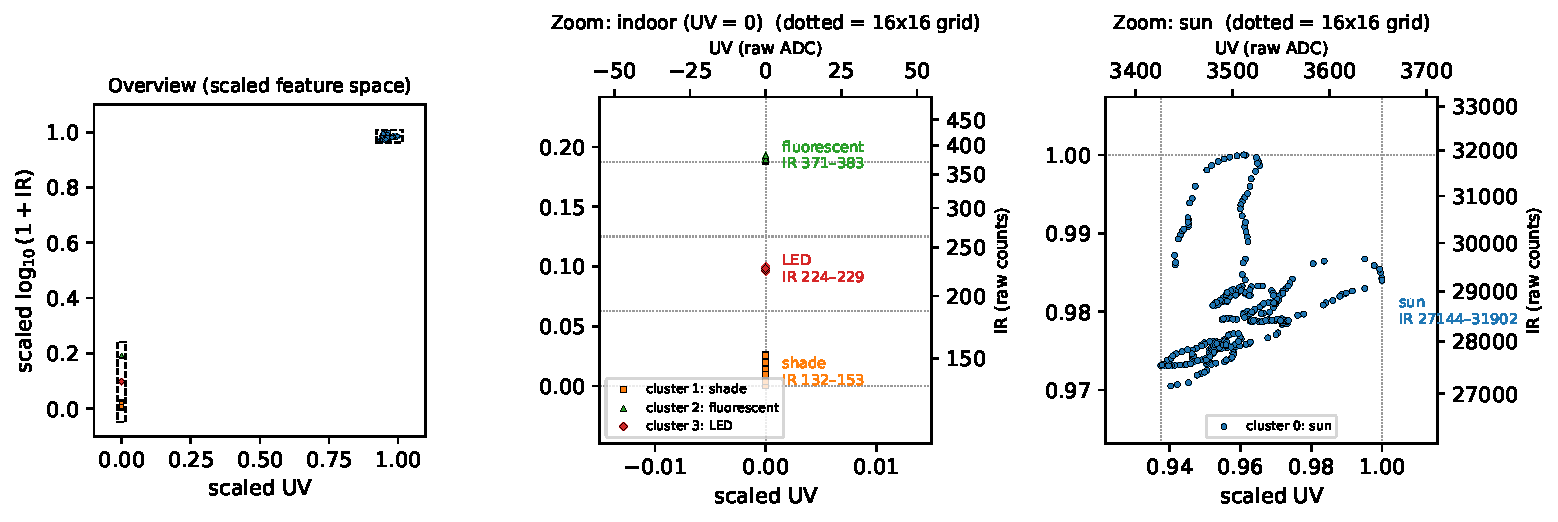
\includegraphics[width=0.95\textwidth]{dbscan_zoom}
\caption{DBSCAN clusters in the scaled feature space. Left: overview. Centre: the three indoor classes, all at UV $=0$, separated only by IR. Right: the sun cluster, whose loops are clouds passing during the recording. Dotted lines are the edges of the $16\times16$ lookup grid; raw sensor units are on the top and right axes.}
\label{fig:zoom}
\end{figure*}

The same figure also shows where the clustering could disagree with the labels in other conditions. The indoor classes differ only in IR brightness, which depends on the distance to the light as much as on its type, so a closer LED or a dimmer fluorescent tube could fall into another class's band. This is a property of the data, not of DBSCAN.

\subsection{Stored model and footprint}

Fig.~\ref{fig:stored} shows the four maps after storage on the $16\times16$ grid. Each class occupies only one or two cells; 250 of the 256 cells (97.7\%) have every class below $\tau$ and answer UNKNOWN. The worst-case \texttt{uint8} quantization error was 0.192\% of peak, within the $1/(2\cdot255) \approx 0.196\%$ bound.

\begin{figure}[!bt]
\centering
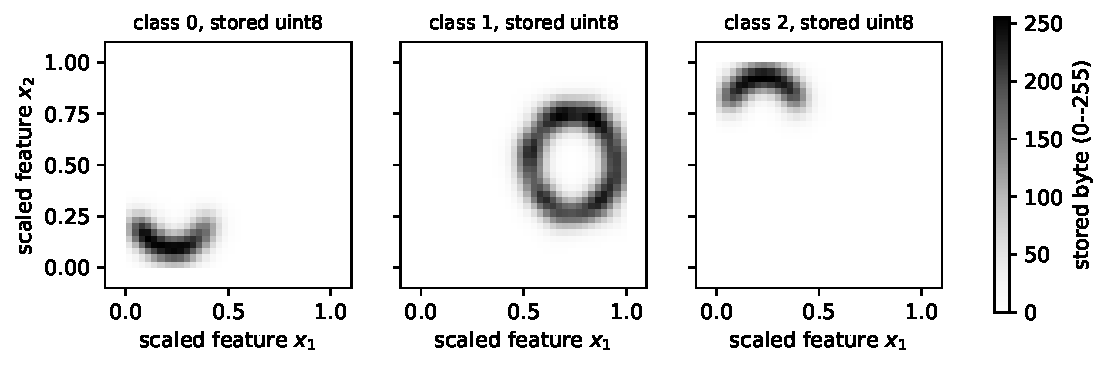
\includegraphics[width=\linewidth]{class_surfaces_discretized}
\caption{The four class maps as stored \texttt{uint8} tables on the $16\times16$ grid. Each class occupies one or two cells; every other cell is below $\tau$.}
\label{fig:stored}
\end{figure}

\begin{table}[!bt]
\centering
\small
\caption{Model footprint by storage format, four classes, $16\times16$ grid. The 16-byte scaling bounds are added to every row.}
\label{tab:footprint}
\begin{tabularx}{\linewidth}{@{}X r r r@{}}
\toprule
Storage & Bytes/cell & Per class & All 4 classes \\
\midrule
\texttt{uint8}   & 1 & 256  & 1024 \\
\texttt{uint16}  & 2 & 512  & 2048 \\
\texttt{float32} & 4 & 1024 & 4096 \\
\texttt{float64} & 8 & 2048 & 8192 \\
\bottomrule
\end{tabularx}
\end{table}

The shipped model is therefore
\begin{equation}
K G^2 + 16 = 4\cdot 16^2 + 16 = 1040\ \text{bytes}.
\label{eq:flash}
\end{equation}

On the 460 test points, which were never used to build or tune the model, the stored \texttt{uint8} lookup agreed with the continuous KDE on 100\% of points (115 per class, no UNKNOWN). Because the labels exist for this dataset, the same test points were also checked against them: all 460 were classified correctly.

\subsection{Readings outside the training data}

Three synthetic queries probe what the reject threshold does. A reading with bright IR but no UV (IR $=3000$, as from a halogen lamp) and a reading with UV but little IR (UV $=2000$, IR $=400$) both returned UNKNOWN, as they should. A reading between LED and fluorescent (IR $=300$), however, returned fluorescent: the gap between those classes is narrower than one grid row, so the reject region does not reach into it. Readings darker than shade are also not rejected: the grid index is clipped into the bottom row, which belongs to shade. On the device, a dark room (IR $\approx 32$) was reported as shade with full score.

\subsection{On-device results}

Sixty held-out readings were logged in full: the last 19--22 readings of each recording, after the sensor had been placed and held still. Feeding the same filtered readings through the Python lookup reproduced the ESP32's decision on all 60 (100\% device-versus-desktop agreement), which confirms that the firmware's feature transform, scaling, rounding, and table layout match the desktop model exactly. On these readings the device also matched the recorded label every time (Table~\ref{tab:heldout}).

That figure overstates the held-out accuracy, and the firmware's own running counts show why. Over the full recordings, the prediction matched the label on only 26 of 75 shade readings (35\%) and 42 of 100 LED readings (42\%), and a longer shade recording, captured in the demonstration video, ended with 504 of 1040 readings matching (48\%). The mismatches came from readings taken while the sensor was being moved or its distance adjusted, so the light reaching it did not represent the labelled condition; the video shows one such stretch, where the sensor was under fluorescent light (IR $\approx 400$) while the recording was still labelled shade, and the device correctly reported fluorescent. The held-out test therefore measured the operator as much as the model. A cleaner protocol, placing the sensor first and starting the recording only once the readings are steady, is part of the remaining work.

Two further caveats apply. The ``shade'' recording was made indoors in a dark spot (IR $\approx 11$), not in outdoor shade like the training data (IR 131--153); it was classified as shade only because readings below the training range are clipped into shade's grid cell. The fluorescent readings (IR 398--440) were brighter than in training (371--383) but stayed in fluorescent's cell. No sun readings were recorded for the held-out batch.

\begin{table}[!bt]
\centering
\small
\caption{Held-out batch on the ESP32, fully logged readings only: recorded label (rows) versus device prediction (columns). Sun was not recorded.}
\label{tab:heldout}
\begin{tabular}{@{}lrrrrr@{}}
\toprule
 & sun & shade & fluor. & LED & UNK. \\
\midrule
sun         & -- & -- & -- & -- & -- \\
shade       & 0 & 19 & 0 & 0 & 0 \\
fluorescent & 0 & 0 & 19 & 0 & 0 \\
LED         & 0 & 0 & 0 & 22 & 0 \\
\bottomrule
\end{tabular}
\end{table}

Table~\ref{tab:costs} compares the measured costs with the prediction. The predicted model data is the 1024-byte table plus 16 bytes of bounds; the measured flash difference also includes the lookup code, the \texttt{log10f} call, and the class-name strings, so it is expected to be somewhat larger. Because \texttt{CLASS\_TABLE} and \texttt{SCALE\_BOUNDS} are \texttt{const}, the ESP32 keeps them in flash, so the predicted SRAM cost is only the 16-byte \texttt{CLASS\_NAMES} pointer array. The lookup itself is four byte reads, one logarithm, and two divisions, so it should take a few microseconds; a full sample is dominated by the TSL2591's 100~ms integration time.

\begin{table}[!bt]
\centering
\small
\caption{Predicted versus measured cost on the ESP32.}
\label{tab:costs}
\begin{tabularx}{\linewidth}{@{}X r r@{}}
\toprule
Quantity & Predicted & Measured \\
\midrule
Flash (model) & 1040 B & 2376 B \\
SRAM (model)  & $\approx$16 B & 20 B \\
Time per lookup & a few \textmu s & 3.26 \textmu s \\
Time per full sample & $\approx$100 ms & 122 ms \\
\bottomrule
\end{tabularx}
\end{table}

The firmware compiled to 294{,}053 bytes of flash and 22{,}028 bytes of SRAM with the model, and 291{,}677 and 22{,}008 bytes without it. The SRAM difference of 20 bytes matches the prediction: the table and bounds stayed in flash, and only the 16-byte \texttt{CLASS\_NAMES} pointer array, plus alignment, landed in RAM. The flash difference of 2376 bytes is 1336 bytes more than the 1040 bytes of model data because enabling the model also links the lookup code, the \texttt{log10f} routine from the maths library, the class-name strings, and the start-up message that reports the model size; the table itself is still the largest single item, and the whole model is 0.18\% of the 1.3~MB program space. Over 1000 lookups the average was 3.26~\textmu s, consistent with four byte reads, one logarithm, and two divisions on a 240~MHz core. A complete sample took 122~ms, slightly more than the TSL2591's 100~ms integration time because of I\textsuperscript{2}C transfer and the ADC read, so the classifier accounts for about 0.003\% of each sample and the sensor sets the achievable rate of about 8~Hz.

% =====================================================================
\section{Filtering Evidence}
\label{sec:filter}

Fig.~\ref{fig:filter} plots the raw and filtered signals against sample index for each condition in the held-out batch. The clearest evidence is at the end of each recording, where the sensor was moved before the recording was stopped. Under shade, raw IR jumped in one sample from 11 to 427 counts, a level that belongs to fluorescent light; the filtered value rose only to 96, which is still inside shade's grid cell, so the reported class did not change. Under LED light a jump from 234 to 306 moved the filtered value only to 246, again without changing the class. These single-sample jumps are exactly the kind of transient the filter is meant to absorb. Across each logged recording, the standard deviation of the sample-to-sample change in IR dropped from 15.7 to 3.3 counts under LED light, from 41.7 to 12.8 under fluorescent light, and from 95.8 to 19.6 in shade (the fluorescent and shade figures include the final jump), a three- to five-fold reduction. A sustained change does pass through: as the fluorescent IR drifted from about 436 down to about 400 counts, the filtered value followed it, lagging by a few samples.

Equally important is what the filter does not remove. The class levels, about 140, 226, and 380 counts for shade, LED, and fluorescent, are separated by far more than the filtered noise, so the filter preserves every class difference the model relies on. Slow changes also pass through: the steady drift of shade IR from 131 to 153 during training, and the cloud-driven swings of sun IR between 27{,}000 and 32{,}000, both appear in the filtered data. They are real changes in the light, not noise.

\begin{figure*}[!t]
\centering
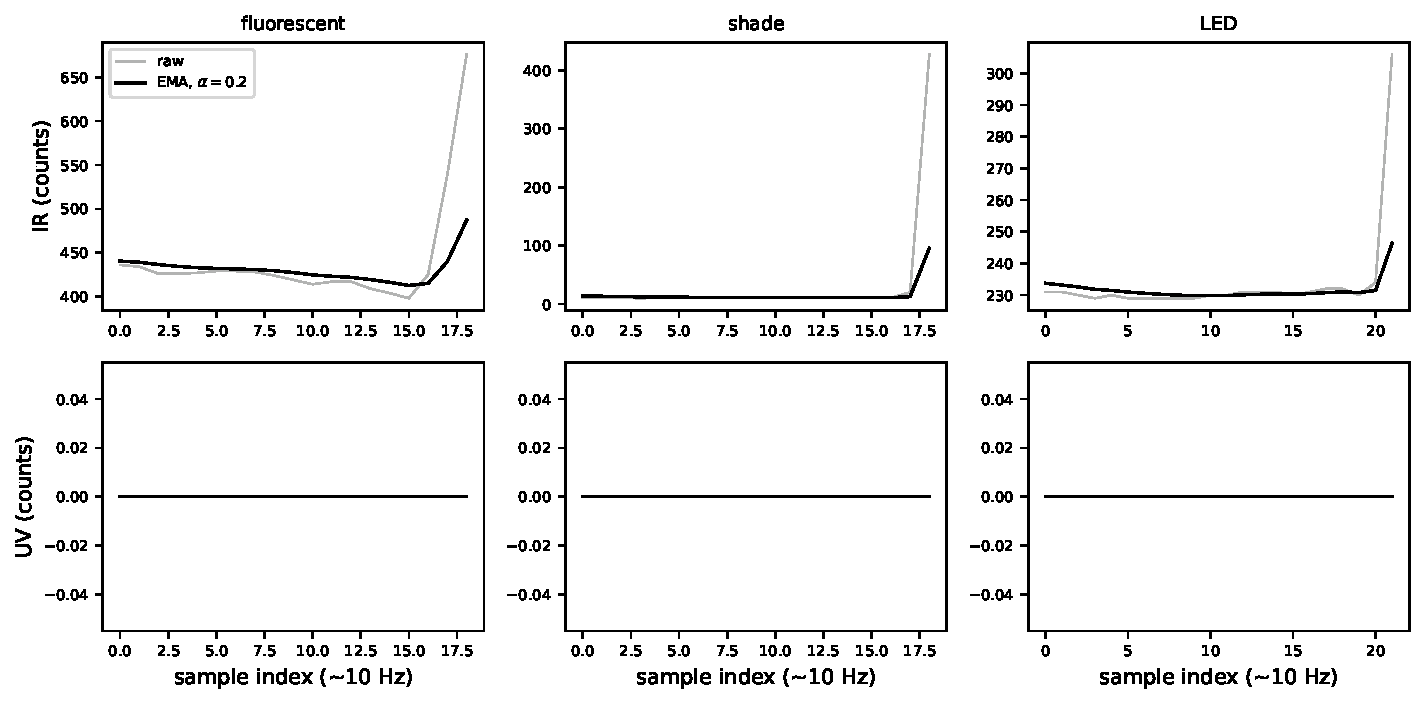
\includegraphics[width=0.95\textwidth]{raw_vs_filtered}
\caption{Raw (grey) and EMA-filtered ($\alpha=0.2$, black) signals versus sample index for each condition of the held-out batch. Top: IR; bottom: UV.}
\label{fig:filter}
\end{figure*}

% =====================================================================
\section{Proof of Concept}

Fig.~\ref{fig:board} shows the wired prototype: the ESP32 with the GUVA-S12SD UV module on GPIO34 and the TSL2591 on the I\textsuperscript{2}C bus. A 35-second video of live classification, showing the serial output updating as the lighting changes, is available at \url{\VIDEOURL}.

\begin{figure}[!bt]
\centering
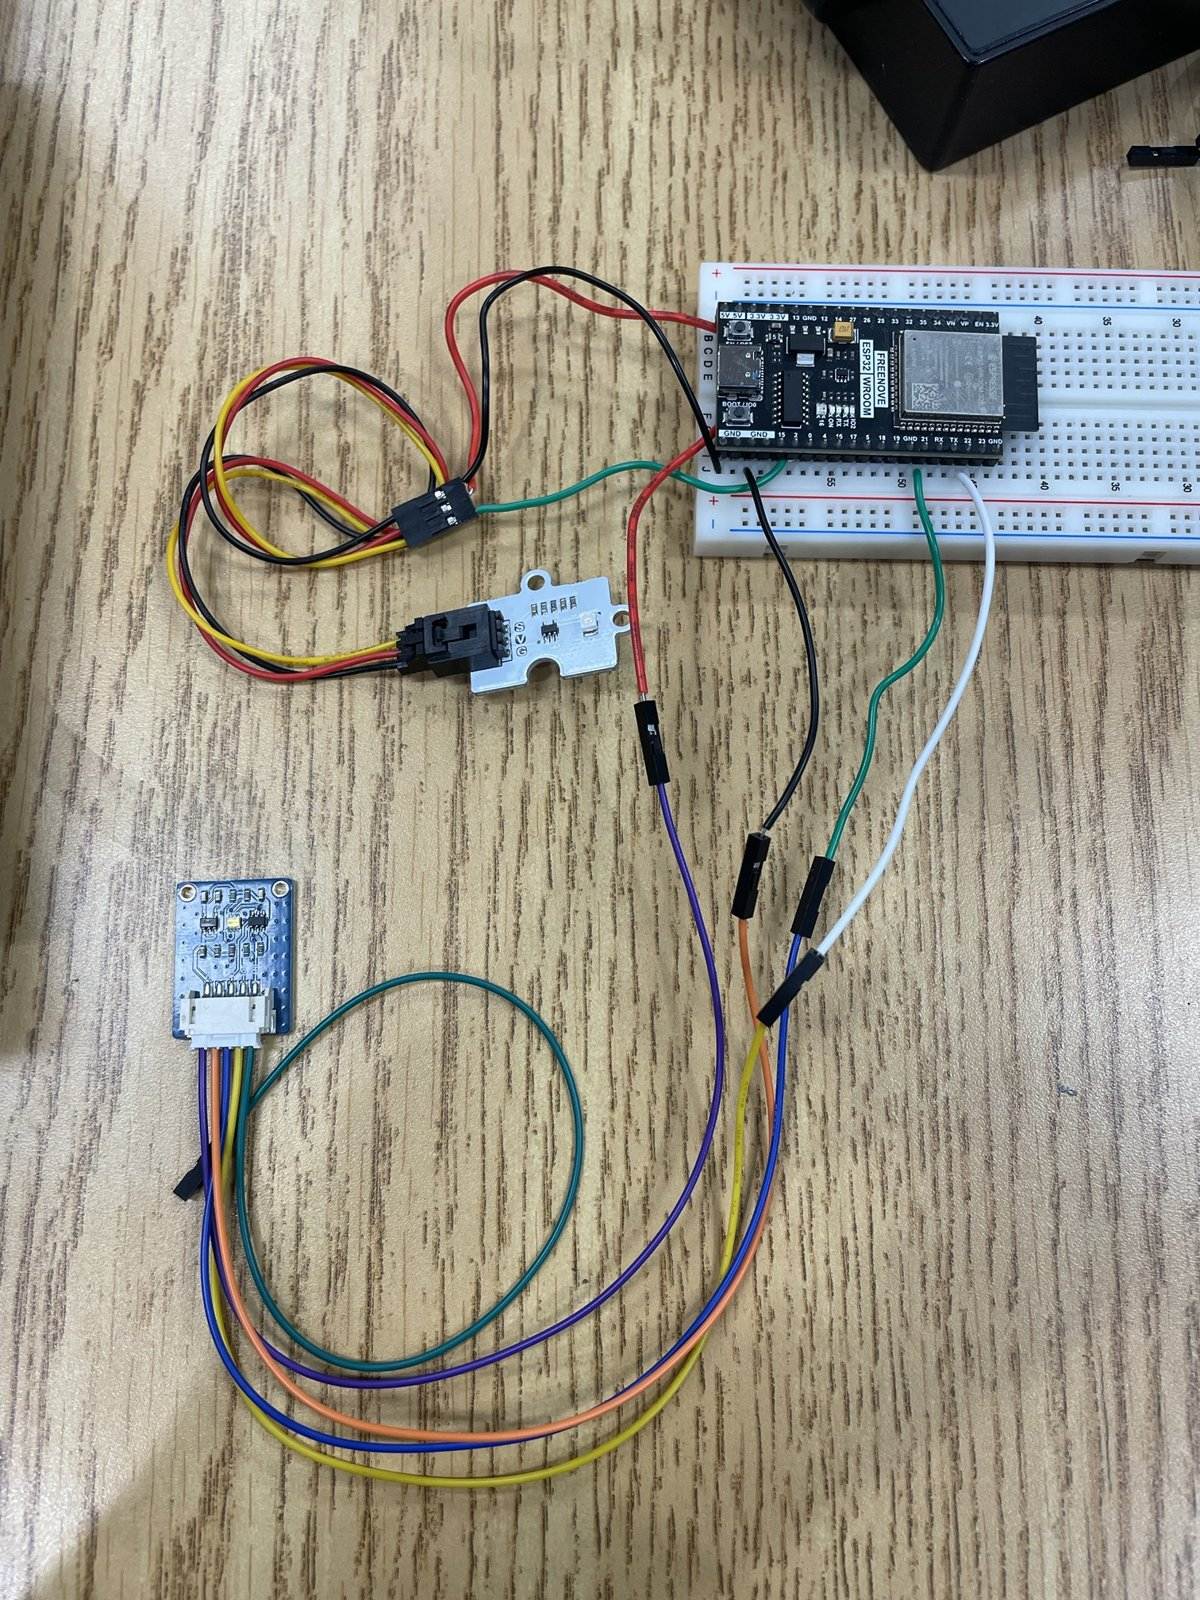
\includegraphics[width=0.75\linewidth]{board_photo}
\caption{The prototype: ESP32, GUVA-S12SD UV module, and TSL2591 light sensor.}
\label{fig:board}
\end{figure}

% =====================================================================
\section{Limitations and Remaining Uncertainty}

The previous lab's main uncertainty was whether the pipeline would hold up on real data with independently established labels. That question is now partly answered: on real sensor data, DBSCAN's clusters matched the recorded labels exactly, the stored tables reproduced the continuous model, and the model ran on the device. What remains uncertain is narrower and more specific to this sensor setup.

\paragraph{The indoor classes are separated by brightness, not by spectrum.} UV is zero for all three indoor classes, so shade, LED, and fluorescent differ only in IR intensity. Intensity depends on distance and angle as much as on the type of light, so the classifier identifies ``an IR level typical of this LED at this distance'' rather than ``LED light''. Moving the sensor would move the readings between classes. A feature that does not depend on distance, such as the ratio of IR to the TSL2591's full-spectrum channel, would address this and is the most important next step.

\paragraph{The reject threshold does not cover every gap.} The threshold correctly rejected lighting with no resemblance to any class. It did not reject a reading between LED and fluorescent, because no empty grid row separates those classes from the reading. It also cannot reject readings darker than shade or brighter than the training range, because the grid index is clipped into an edge cell. Rejecting out-of-range readings explicitly, before the lookup, would be a simple fix.

\paragraph{The classes are well separated, so perfect agreement is weak evidence.} The 100\% DBSCAN purity and 100\% test agreement say that these four recordings are easy to separate. They do not show how the pipeline behaves when classes overlap, as they would with more light sources or mixed lighting.

\paragraph{The bandwidth was not selected by a clear optimum.} The validation likelihood rose monotonically toward the smallest bandwidth tested (Table~\ref{tab:bandwidth}), partly because the UV feature is constant indoors and partly because consecutive readings are near-duplicates. A split by recording session rather than by random row would give a more honest validation score.

\paragraph{The held-out test was weaker than planned.} Only the last 19--22 readings of each recording were logged in full, sun was not recorded, and the shade recording was made indoors at a light level below the training range. The running counts over the full recordings (35\% and 42\% agreement with the label for shade and LED) show that readings taken while the sensor is being positioned are frequently misclassified. A repeat with a fixed sensor mount, outdoor sun and shade, and complete logs is needed before the held-out accuracy can be stated with confidence; the device-versus-desktop agreement, by contrast, does not depend on these conditions.

\paragraph{Limited conditions.} Each class comes from one recording session, with one sensor position, so variation in time of day, weather, lamp age, and sensor placement is largely untested. The UV ADC reached about 3650 of 4095 in sun, close to the range where the ESP32 ADC becomes non-linear, so brighter sun could saturate.

Overall, the pipeline worked as proposed on real data and real hardware, with 1040 bytes of model data, 2376 bytes of total flash cost, and a lookup time of 3.26~\textmu s. The next step is to make the features independent of sensor distance and to test with more light sources and recording sessions.

\end{document}